% ===== Section 5 (Alex). Replaces everything from \textbf{(a) Data collection.} to the end of (e). =====
% Every number below is written by scripts/06_eda.py to results/eda/*.csv (file named in each % comment).
\textbf{(a) Data collection.} \emph{Inspections:} state survey agencies, working for CMS, run unannounced standard surveys of every certified facility (federally required at most 15 months apart) and investigate complaints in between; each violation cited is a deficiency. \emph{Staffing and turnover} come from the Payroll-Based Journal (PBJ), payroll data that facilities submit quarterly \TODO{confirm which PBJ quarter the Oct 2026 file uses}. \emph{Ratings} come from CMS's five-star methodology \TODO{confirm current inspection-cycle weights}. Issues for us: staffing, census and turnover are self-reported administrative data; current inspections date from 2019-10-03 to 2026-09-23 (1.1\% before 2023) while staffing is recent, so predictors can postdate the inspection; inspector strictness differs by state; 69\% of facilities belong to one of 611 chains, so rows are clustered (Lecture 10); and complaint deficiencies arise only if someone files a complaint.
% dataset_facts.csv

\textbf{(b) Correlations with the outcome.} The outcome is right-skewed (mean 9.17, median 7, SD 8.07, skewness 1.99, 5.2\% zeros; Figure~1a), so Pearson $r$ is partly driven by the tail. Inspection history is most strongly associated with it (Figure~1b): prior-cycle deficiencies $r=0.62$, prior complaint deficiencies $0.52$. The strongest non-history features are RN turnover ($0.24$), log beds ($0.21$) and administrator departures ($0.20$). Surprisingly, staffing \emph{levels} are weak: total nurse hours $r=-0.14$, RN hours $-0.15$. The weakest are occupancy ($0.01$), LPN hours ($0.05$) and PT hours ($-0.06$). Mean deficiencies are 10.1 for for-profit vs.\ 6.3 non-profit and 7.1 government facilities (Figure~1c), 9.7 in chains vs.\ 7.9 independent, 9.8 urban vs.\ 7.5 rural, and range from 2.7 (AR) to 17.1 (NM) across states with at least 20 facilities (Figure~1d).
% outcome_summary.csv, corr_with_outcome.csv, categorical_outcome.csv, state_means.csv

\textbf{(c) Correlations among covariates.} Several features are near-duplicates: prior deficiency score vs.\ prior total health score ($r=0.98$), weekday vs.\ weekend nurse hours ($0.98$), RN vs.\ weekend RN hours ($0.95$), beds vs.\ residents ($0.92$). This collinearity inflates OLS variance, one reason we also fit lasso (Lecture 7). Ownership and chains overlap: 80\% of for-profits are in a chain vs.\ 40\% of non-profits and 38\% of government facilities.
% top_feature_pairs.csv, crosstab_ownership_chain.csv

\textbf{(d) Subgroups.} Compared with non-profits, for-profits report fewer nurse hours (3.72 vs.\ 4.47 per resident-day) and RN hours (0.62 vs.\ 0.95), higher turnover (46.5\% vs.\ 41.1\%) and case mix (1.43 vs.\ 1.31), and more prior deficiencies (14.1 vs.\ 8.0). Chain facilities differ from independents in the same direction (3.74 vs.\ 4.29 nurse hours; 13.5 vs.\ 10.4 prior deficiencies). Urban facilities are larger than rural ones (115 vs.\ 85 beds) with similar staffing (3.94 vs.\ 3.81 hours), yet have more prior (13.6 vs.\ 9.8) and current (9.8 vs.\ 7.5) deficiencies. Groups differ on several covariates at once, so no single comparison isolates ownership, chain or location.
% subgroup_means.csv

\textbf{(e) Missing values.} We drop the 31 rows (0.3\%) with a missing outcome, leaving 11{,}717; they are also the only rows missing inspection history. Missingness in the remaining features is modest: RN turnover 12.5\%, administrator departures 11.0\%, nursing turnover 7.1\%, family council 5.1\%, staffing and case mix 2.4\%, beds and residents under 0.5\%. We impute rather than drop because 22\% of facilities miss at least one feature and they differ in composition (68\% for-profit vs.\ 75\% of complete rows), so dropping would lose facilities non-randomly. Numeric features get median imputation plus a missing-indicator column; categorical features get the most frequent level. Both are fit inside each CV training fold within the \texttt{Pipeline} (Lecture 4: imputation must be fit inside each training fold). Of the 24 columns over 30\% missing, the 15 footnote codes are dropped, the 7 chain fields (blank for non-chain facilities) are coded explicitly (chain membership = no, chain size = 1), and the 2 inspection-derived ones are excluded as leakage.
% missingness_fs2.csv, dataset_facts.csv, missing_over30_by_type.csv

% ===== Section 6(d): replace the OLS bullet (the one ending in \TODO{Alex}) =====
  \item \textbf{OLS linear regression:} predicts $\hat y = \hat\beta_0 + x^\top\hat\beta$, with $\hat\beta$ chosen to minimize the sum of squared residuals on the training fold (Lecture 2). It is our interpretable benchmark: each coefficient is an association holding the other features fixed, and under a correct linear model with uncorrelated, equal-variance errors it has the lowest variance among linear unbiased estimators (Gauss--Markov, Lecture 7), so lasso and the random forest must beat it to justify their added bias or complexity.

% ===== Figures page: replace the \TODO{...} line under \section*{Figures} =====
\begin{figure}[h]\centering
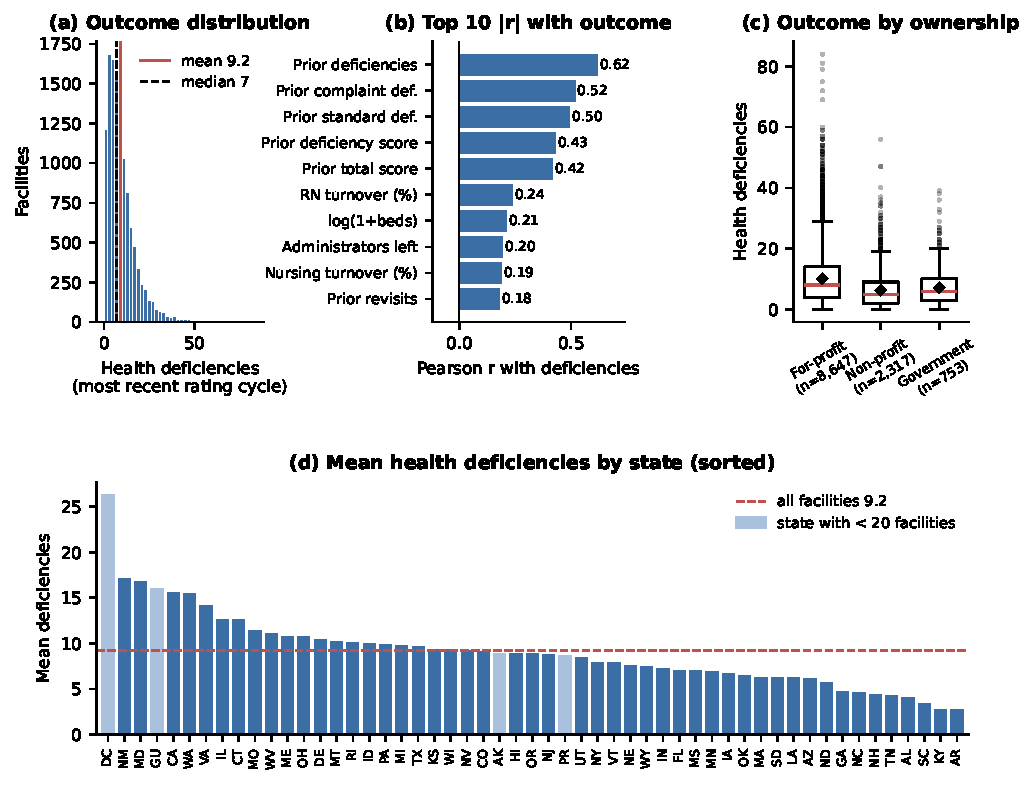
\includegraphics[width=\linewidth]{figures/fig1.pdf}
\caption{Development data ($n=11{,}717$): (a) outcome distribution; (b) the 10 numeric features with the largest $|r|$ with the outcome; (c) outcome by ownership (diamond = mean); (d) mean deficiencies by state (light bars: fewer than 20 facilities).}
\end{figure}
